\documentclass[10pt,a4paper]{article}
\usepackage[margin=2.2cm]{geometry}
\usepackage{fontspec}
\usepackage{kotex}
\setmainfont{Apple SD Gothic Neo}
\setsansfont{Apple SD Gothic Neo}
\usepackage{amsmath,amssymb}
\usepackage{graphicx}
\usepackage{booktabs}
\usepackage{caption}
\usepackage[dvipsnames]{xcolor}
\usepackage[colorlinks=true,linkcolor=MidnightBlue,citecolor=MidnightBlue,
            urlcolor=MidnightBlue]{hyperref}
\usepackage{titlesec}
\titleformat{\section}{\large\bfseries}{\thesection}{0.6em}{}
\titleformat{\subsection}{\normalsize\bfseries}{\thesubsection}{0.5em}{}
\captionsetup{font=small,labelfont=bf}
\setlength{\parskip}{0.35em}
\setlength{\parindent}{0pt}

\usepackage{mdframed}
\newmdenv[linewidth=0.4pt,linecolor=gray!60,backgroundcolor=gray!5,
          innertopmargin=6pt,innerbottommargin=6pt,skipabove=8pt,skipbelow=8pt]{claimbox}
\newcommand{\claim}[2]{\begin{claimbox}\textbf{주장.} #1\par\smallskip
  \textcolor{gray!70}{\textbf{반증 조건.} #2}\end{claimbox}}

\title{\bfseries U 자를 놓쳤다\\[2pt]
\large 날짜 상관이 $-0.001$ 인 계열이 학습과 유보를 완전히 갈랐다 --- 해로움의
$59\%$ 가 그것이었다}
\author{월드모델 실험실 · 노트 757 $\sim$ 762}
\date{2026-08-07}
\begin{document}\maketitle

\section{한 줄}

논문 $148$ 이 \textbf{장의 전국 시간축이 판을 해친다}(신호 몫 $-0.0192$)를 확정하고
기제 후보 하나(방향 뒤집힘)를 지웠다. 여기서 둘을 더 지우고 --- \textbf{거칠기}와
\textbf{남은 하나} --- 원인을 찾았다.

\textbf{그 축의 원천 계열은 날짜와 상관이 $\mathbf{-0.001}$ 이다.} 추세가 전혀 없다.
\textbf{그런데 연도별 중앙값이 U 자다} --- $2020$ $0.00853 \to 2023$ $\mathbf{0.00793}
\to 2026$ $\mathbf{0.00900}$. \textbf{학습($2020{\sim}24$)이 골에 있고 유보($2025{\sim}26$)가
오른쪽 어깨에 있다.} 도메인 안 백분위로 넣었으니 \textbf{학습과 유보의 백분위 분포가
갈렸다 --- 사분위 겹침 $0.074$.}

분포를 맞추니 \textbf{신호 몫이 $-0.0192 \to -0.0079$ 로 $59\%$ 줄었고}, 남은 것은
\textbf{두 도메인에 몰려 있다.}

\section{먼저 거칠기를 지웠다}

논문 $148$ 이 실마리를 남겼다 --- 가장 해로운 둘에서 학습 상관 $0.08$ 이 유보에서
$0.02$ 로 \textbf{감쇠}한다. 그러면 \emph{``약한 신호가 강한 분할 여지를 준다''}가
후보다: 이 축은 날짜에서 왔으므로 고유값이 많다(웹툰 $1{,}594$).

\begin{center}
\begin{tabular}{lrrl}
\toprule
& 순효과 & 원본과의 차 & \\
\midrule
원본 (고유 $1{,}594$) & $0.0284$ & --- & 논문 $148$ \\
고유 $10$ & $0.0240$ & $+0.0044$ & 문턱 $0.010$ 미달 \\
고유 $4$ & $0.0233$ & $+0.0051$ & 문턱 미달 \\
\bottomrule
\end{tabular}
\end{center}

\textbf{단조로 줄지만 폭이 $0.005$ 다.} 고유 $10$ 의 신호 몫은 $-0.0175$ 로 원본
$-0.0192$ 와 거의 같다. \textbf{거칠기가 아니다.}

\claim{\textbf{논문 $146$ 의 결과를 다른 시험대에 옮긴 것이 내 실수였다.} 그 논문은
\textbf{완전관측 순수 난수} 열에서 ``거친 열이 덜 비싸다''를 쟀다($0.0015$/열 폭).
나는 그것을 \textbf{부분관측 · 실제 축}에 그대로 적용해 예측했고 $10{\sim}25$배
틀렸다. \textbf{규약 $18$(가드를 인용할 때 시험대를 적는다)을 내가 세우고 내가
어겼다.}}
{거칠기 효과가 실재하지만 이 축에서는 다른 것에 가려진 것일 수도 있다 --- 아래 공변량
이동을 제거한 뒤에 거칠기를 다시 재면 보일 수 있다. \textbf{그 조합은 안 쟀다.}}

\section{그리고 U 자를 찾았다}

\begin{figure}[t]\centering
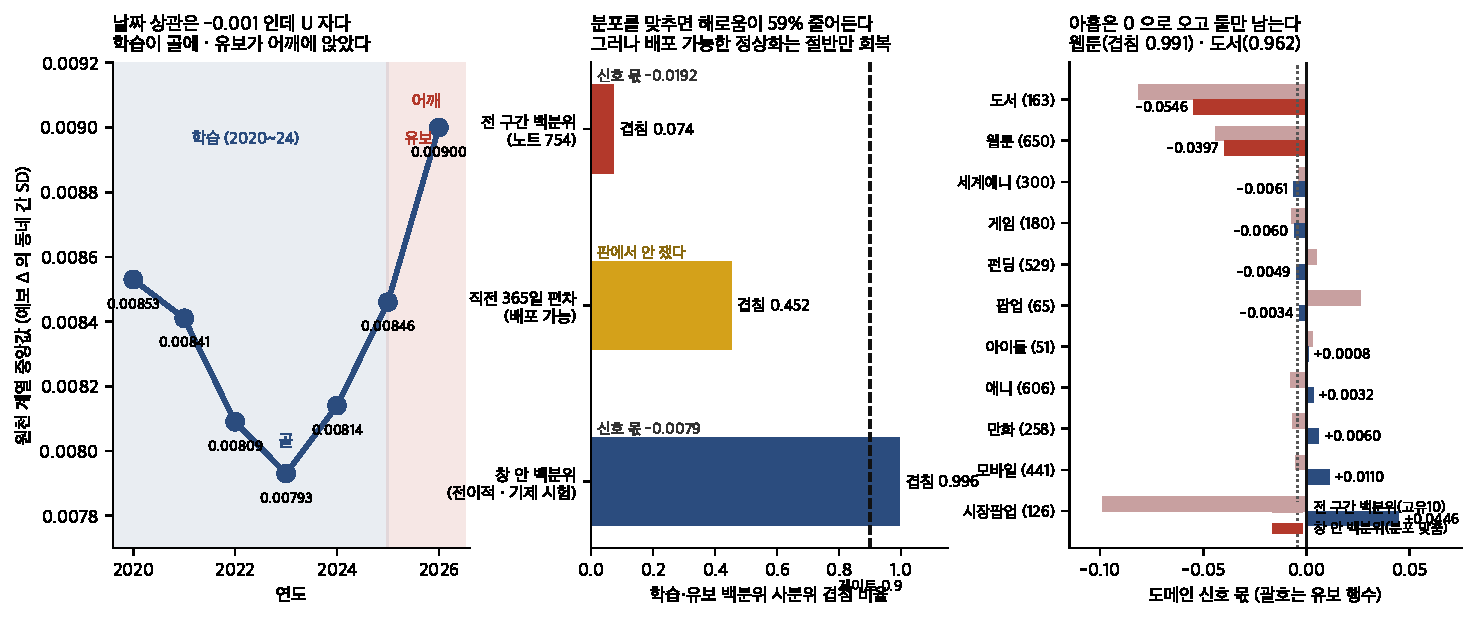
\includegraphics[width=0.99\textwidth]{figs/ushape.pdf}
\caption{왼쪽: \textbf{날짜 상관이 $-0.001$ 인데 U 자다} --- 학습이 골에, 유보가
어깨에 앉았다. 가운데: \textbf{분포를 맞추면 해로움이 $59\%$ 줄지만} 배포 가능한
정상화는 절반만 회복한다. 오른쪽: \textbf{아홉은 $0$ 으로 오고 둘만 남는다.}}
\end{figure}

논문 $148$ 은 \textbf{축$\leftrightarrow$날짜 스피어만}으로 시간 결함을 검사하고
\emph{``깨끗하다''}고 판정했다 --- 판 기여 $1$위 웹툰이 $0.071$ 이었다.
\textbf{그 검사가 틀렸다.}

\begin{center}
\begin{tabular}{lr}
\toprule
원천 계열 $\leftrightarrow$ 날짜 스피어만 & $\mathbf{-0.001}$ ($p=0.956$) \\
\midrule
$2020$ 중앙값 & $0.00853$ \\
$2022$ & $0.00809$ \\
$2023$ & $\mathbf{0.00793}$ \quad (골) \\
$2024$ & $0.00814$ \\
$2025$ & $0.00846$ \\
$2026$ & $\mathbf{0.00900}$ \quad (어깨) \\
\bottomrule
\end{tabular}
\end{center}

\claim{\textbf{시간 결함은 단조 상관이 아니라 창별 분포로 검사한다.} U 자 계열은
\textbf{단조 상관이 정확히 $0$ 이면서도 학습과 유보를 완전히 가른다.} 도메인 안
백분위 사분위 겹침 중앙값이 \textbf{$0.074$} 였다 --- 학습이 $[0.19, 0.63]$ 에 있고
유보가 $[0.54, 0.91]$ 에 있으면(웹툰) 트렁크는 \textbf{라벨과 함께 본 적 없는
구간에서} 예보한다.}
{겹침이 낮아도 관계가 매끄러우면 외삽이 잘 될 수 있다. \textbf{그러나 이 축의
관계는 $|$상관$| \approx 0.05$ 로 약하다} --- 약한 관계를 못 본 구간으로 외삽하는
것이 위험한 조합이다. 겹침만으로 판정하면 매끄러운 축을 억울하게 버릴 수 있으므로
\textbf{겹침은 경보이고 판정은 판에서 한다.}}

\section{분포를 맞추니 $59\%$ 가 사라졌다}

\textbf{창 안 백분위}로 다시 만들었다 --- 학습 행은 학습 안에서, 유보 행은 유보
안에서 순위. 그러면 두 분포가 구성상 같다(\textbf{겹침 중앙값 $0.996$}).

\begin{center}
\begin{tabular}{lrrr}
\toprule
& 없이 & 진짜 & 위약 $3$뽑기 평균 \\
\midrule
판 & $0.4685$ & $\mathbf{0.4515}$ & $0.4594$ (뽑기 SD $0.0029$) \\
\midrule
& \multicolumn{3}{l}{\textbf{신호 몫 $-0.0192 \to \mathbf{-0.0079}$} ($59\%$ 개선) ·
순효과 $-0.0284 \to -0.0170$} \\
\bottomrule
\end{tabular}
\end{center}

\textbf{사전등록 규칙 (나) 발동 --- 절반쯤 기제다.} 사전등록 예측은 \emph{``신호 몫
$-0.008 \sim +0.006$''}였고 \textbf{$-0.0079$ 로 하단에 맞았다.}

\subsection*{🔴 이것은 채택이 아니다 --- 미리 적어 뒀다}

\textbf{창 안 백분위는 전이적이다} --- 유보 행을 유보 행들 사이에서 순위 매긴다.
라벨은 안 보지만 \textbf{유보의 주변 분포를 쓴다.} 그래서 \textbf{기제 시험 전용}이고
채택 축이 아니다(사전등록에 미리 적었다).

배포 가능한 후보로 \textbf{직전 $365$일 중앙값을 뺀 편차}를 재 봤다 --- \textbf{겹침
$0.074 \to 0.452$ 로 절반만 회복}한다(유보 중앙차 $0.366 \to 0.316$). \textbf{U 자가
느린 추세가 아니라 $2025{\sim}26$ 산포가 자기 직전 $1$년 대비로도 높기 때문}이다.

\claim{\textbf{전 구간 백분위는 편차를 다시 수준으로 되돌린다.} 노트 $646$ 이
\emph{``범도메인 시간축은 수준이 아니라 편차여야 한다''}를 세웠는데, \textbf{편차로
만든 값을 학습 $+$ 유보 전 구간 백분위로 넣으면 창별 분포가 갈려 다시 수준이 된다.}
정규화의 한 단계가 앞 단계의 통제를 지운다.}
{$0.996$ 과 $0.074$ 의 차이가 판에서 $59\%$ 를 냈다는 것이 이 주장의 근거다. 그러나
\textbf{창 안 백분위는 분포만 바꾸는 것이 아니라 순위 자체를 바꾼다} --- 그 두 효과를
이 실험은 못 가른다. 가르려면 \textbf{분포는 맞추되 순위를 보존하는} 변환(학습 CDF
로 사상 $+$ 유보 재중심)이 필요하고, 안 했다.}

\section{남은 $41\%$ 는 두 도메인에 몰려 있다}

\begin{center}
\begin{tabular}{lrrr|lrrr}
\toprule
도메인 & 신호 몫 & 겹침 & 유보 & 도메인 & 신호 몫 & 겹침 & 유보 \\
\midrule
\textbf{도서} & $\mathbf{-0.0546}$ & $0.962$ & $163$ & 팝업 & $-0.0034$ & $0.960$ & $65$ \\
\textbf{웹툰} & $\mathbf{-0.0397}$ & $0.991$ & $650$ & 아이돌 & $+0.0008$ & $1.000$ & $51$ \\
세계애니 & $-0.0061$ & $1.000$ & $300$ & 애니 & $+0.0032$ & $0.997$ & $606$ \\
게임 & $-0.0060$ & $0.994$ & $180$ & 만화 & $+0.0060$ & $1.000$ & $258$ \\
펀딩 & $-0.0049$ & $1.000$ & $529$ & 모바일 & $+0.0110$ & $1.000$ & $441$ \\
& & & & 시장팝업 & $+0.0446$ & $0.740$ & $126$ \\
\bottomrule
\end{tabular}
\end{center}

\textbf{아홉 도메인이 문턱($0.0045$) 근처로 왔고 웹툰 · 도서만 남는다.} 그 둘이 판
기여 $-0.00766$ · $-0.00264$ 로 전체를 끌어내린다. \textbf{그리고 그 둘의 겹침이
$0.991 \cdot 0.962$ 로 완벽하다} --- 공변량 이동이 아니다.

\textbf{시장팝업이 $-0.0987 \to +0.0446$ 로 부호를 뒤집었다.} 다만 그 도메인은 축
고유값이 $5$ 개(행 날짜가 연 단위)라 겹침 게이트에서 면제한 도메인이므로
\textbf{근거로 쓰지 않는다.}

\claim{\textbf{남은 것은 국소적이다} --- 그러나 아직 확정이 아니다. \textbf{다음
실험이 그것을 시험한다}: 웹툰 · 도서를 빼고 다시 재서 \textbf{신호 몫이 문턱 안으로
들어오면} 국소가 확정되고, 물음이 \emph{``그 둘의 공통점은 무엇인가''}로 좁아진다.
\textbf{눈에 보이는 공통점 하나} --- 둘 다 \textbf{연재물}이고 라벨이 누적형이다.
시점 상태와 누적 라벨이 안 맞을 수 있다.}
{빼고 재서 문턱 안으로 안 들어오면 국소가 아니라 전역이고, 그때는 축 자체를 버린다.
그리고 \textbf{두 도메인을 빼는 것 자체가 표본을 고르는 것}이므로 --- 빼면 판이
좋아지는 것은 당연할 수 있다 --- \textbf{판정은 그 둘을 뺀 판에서의 신호 몫}으로
하고 절대 수준은 안 본다.}

\section{배선을 한 번 고쳤다 --- 면제를 숨기지 않았다}

겹침 게이트($<0.9$ 면 중단)가 \textbf{시장팝업($0.740$)} 에서 멈췄다. 그 도메인은
고유값 $5$ 개라 \textbf{창 안 백분위로도 사분위가 겹칠 수 없다.} 그래서 \textbf{고유값
$6$ 이하 도메인(시장팝업 $5$ · 아이돌 $6$ · 펀딩 $6$)을 겹침 게이트에서 면제}하고
\textbf{산출에 목록을 찍게} 고쳤다.

\claim{\textbf{게이트를 느슨하게 한 것이 아니라 대상을 정확히 한 것이다} --- 애초에
정보를 못 나르는 도메인에 분포 겹침을 요구할 수 없다. \textbf{그리고 면제는 반드시
산출에 남긴다} --- 안 남기면 다음 사람이 ``$11$ 도메인 전부 겹침 $0.9$ 이상''으로
읽는다.}
{면제 기준($6$)이 내 눈이 정한 값이다. 자료가 정하게 하려면 \textbf{고유값 $\div$
행수} 같은 비율을 쓰거나 \textbf{겹침을 계산할 수 있나}를 직접 판정해야 한다.
$6$ 은 관측된 세 도메인의 값($5 \cdot 6 \cdot 6$)에서 왔으므로 \textbf{자료를 보고
정한 문턱}이고, 그것을 적어 둔다.}

\end{document}
